%%%%%%%%%%%%%%%%%%%%%%%%%%%%%%%%%%%%%%%%%%%%%%%%%%%%%%%%%%%%%%%%%%%%%%%%%%%%%%%
% CASE STUDY TEMPLATE - Programming and Problem Solving
% Author: Brendan Shea, PhD
% Course: Programming and Problem Solving
% Rochester Community and Technical College
%%%%%%%%%%%%%%%%%%%%%%%%%%%%%%%%%%%%%%%%%%%%%%%%%%%%%%%%%%%%%%%%%%%%%%%%%%%%%%%

\documentclass[11pt,letterpaper]{article}

%---------- PACKAGES ----------%
\usepackage[margin=1in, headheight=22pt]{geometry}
\usepackage[T1]{fontenc}
\usepackage{xcolor}
\usepackage{tcolorbox}
\usepackage{graphicx}
\usepackage{titlesec}
\usepackage{enumitem}
\usepackage{fancyhdr}
\usepackage{listings}
\usepackage{hyperref}
\usepackage{multicol}
\usepackage{booktabs}
\usepackage{tikz}
\usepackage{float}
\usepackage{amssymb}
\usepackage{amsmath}
\usepackage{pifont}

% TikZ libraries
\usetikzlibrary{shapes.geometric, arrows.meta, positioning, calc,
                backgrounds, fit, matrix, decorations.pathreplacing, chains}

% Load tcolorbox libraries
\tcbuselibrary{skins,breakable,listings,listingsutf8}

%---------- COLOR DEFINITIONS ----------%
\definecolor{csprimary}{HTML}{2C3E50}
\definecolor{cssecondary}{HTML}{E74C3C}
\definecolor{cstertiary}{HTML}{3498DB}
\definecolor{csaccent}{HTML}{27AE60}
\definecolor{cswarm}{HTML}{F39C12}
\definecolor{cslight}{HTML}{ECF0F1}
\definecolor{csdark}{HTML}{1A252F}

% Syntax highlighting colors
\definecolor{codegreen}{HTML}{27AE60}
\definecolor{codepurple}{HTML}{9B59B6}
\definecolor{codeorange}{HTML}{E67E22}
\definecolor{codeblue}{HTML}{3498DB}
\definecolor{codegray}{HTML}{95A5A6}
\definecolor{codestring}{HTML}{E74C3C}
\definecolor{codebg}{HTML}{1E2A38}

%---------- CASE STUDY METADATA ----------%
\newcommand{\cstitle}{The Moth in the Machine}
\newcommand{\cssubtitle}{A History of Software Bugs and the Science of Testing}
\newcommand{\csauthor}{Brendan Shea, PhD}
\newcommand{\cscourse}{Programming and Problem Solving}
\newcommand{\csinstitution}{Rochester Community and Technical College}
\newcommand{\csdate}{\today}

%---------- LISTINGS CONFIGURATION ----------%
\lstdefinestyle{basestyle}{
    backgroundcolor=\color{codebg},
    basicstyle=\ttfamily\small\color{white},
    breakatwhitespace=false,
    breaklines=true,
    captionpos=b,
    keepspaces=true,
    showspaces=false,
    showstringspaces=false,
    showtabs=false,
    tabsize=4,
    frame=none,
    xleftmargin=4mm,
    xrightmargin=4mm,
    aboveskip=0pt,
    belowskip=0pt,
}

\lstdefinestyle{javastyle}{
    style=basestyle,
    language=Java,
    keywordstyle=\color{codeblue}\bfseries,
    commentstyle=\color{codegray}\itshape,
    stringstyle=\color{codestring},
    morekeywords={String, Scanner, System, var, boolean, Math, List, Map,
                  HashMap, ArrayList, Test, assertEquals, assertTrue,
                  assertThrows, BeforeEach, assertFalse},
}

%---------- CUSTOM ENVIRONMENTS ----------%
\newcommand{\keyterm}[1]{\textbf{\textcolor{cssecondary}{#1}}}

\newtcolorbox{conceptbox}[1][]{
    enhanced,
    colback=cslight,
    colframe=csprimary,
    fonttitle=\bfseries\color{white},
    title=#1,
    attach boxed title to top left={yshift=-2mm, xshift=5mm},
    boxed title style={colback=csprimary},
    breakable
}

\newtcolorbox{historybox}[1][]{
    enhanced,
    colback=codepurple!8,
    colframe=codepurple,
    fonttitle=\bfseries\color{white},
    title=#1,
    attach boxed title to top left={yshift=-2mm, xshift=5mm},
    boxed title style={colback=codepurple},
    breakable
}

\newtcolorbox{tipbox}[1][]{
    enhanced,
    colback=csaccent!8,
    colframe=csaccent,
    fonttitle=\bfseries\color{white},
    title=#1,
    attach boxed title to top left={yshift=-2mm, xshift=5mm},
    boxed title style={colback=csaccent},
    breakable
}

\newtcolorbox{warningbox}[1][]{
    enhanced,
    colback=cssecondary!8,
    colframe=cssecondary,
    fonttitle=\bfseries\color{white},
    title=#1,
    attach boxed title to top left={yshift=-2mm, xshift=5mm},
    boxed title style={colback=cssecondary},
    breakable
}

\newtcolorbox{debatebox}[1][]{
    enhanced,
    colback=cswarm!8,
    colframe=cswarm,
    fonttitle=\bfseries\color{white},
    title=#1,
    attach boxed title to top left={yshift=-2mm, xshift=5mm},
    boxed title style={colback=cswarm},
    breakable
}

\newtcolorbox{quotebox}[1][]{
    enhanced,
    colback=cstertiary!8,
    colframe=cstertiary,
    fonttitle=\bfseries\color{white},
    title=#1,
    attach boxed title to top left={yshift=-2mm, xshift=5mm},
    boxed title style={colback=cstertiary},
    breakable
}

\newtcblisting{javacode}[1][]{
    enhanced,
    colback=codebg,
    colframe=csaccent,
    colupper=white,
    fonttitle=\bfseries\color{white},
    title=#1,
    attach boxed title to top left={yshift=-2mm, xshift=5mm},
    boxed title style={colback=csaccent},
    left=0mm, right=0mm, top=2mm, bottom=2mm,
    boxrule=1pt,
    breakable,
    pad at break=2mm,
    listing only,
    listing options={style=javastyle}
}

\newtcblisting{bugcode}[1][]{
    enhanced,
    colback=codebg,
    colframe=cssecondary,
    colupper=white,
    fonttitle=\bfseries\color{white},
    title=#1,
    attach boxed title to top left={yshift=-2mm, xshift=5mm},
    boxed title style={colback=cssecondary},
    left=0mm, right=0mm, top=2mm, bottom=2mm,
    boxrule=1pt,
    breakable,
    pad at break=2mm,
    listing only,
    listing options={style=javastyle}
}

\newtcolorbox{questionbox}{
    enhanced,
    colback=cswarm!10,
    colframe=cswarm,
    fonttitle=\bfseries\color{white},
    title=Discussion Questions,
    attach boxed title to top center={yshift=-2mm},
    boxed title style={colback=cswarm},
    breakable
}

\newtcolorbox{glossarybox}{
    enhanced,
    colback=cslight,
    colframe=csprimary,
    fonttitle=\bfseries\color{white},
    title=Glossary of Key Terms,
    attach boxed title to top center={yshift=-2mm},
    boxed title style={colback=csprimary},
    breakable
}

%---------- HEADER/FOOTER ----------%
\pagestyle{fancy}
\fancyhf{}
\fancyhead[L]{\small\textcolor{csprimary}{\cscourse}}
\fancyhead[R]{\small\textcolor{csprimary}{Case Study}}
\fancyfoot[C]{\thepage}
\renewcommand{\headrulewidth}{0.4pt}
\renewcommand{\headrule}{\hbox to\headwidth{\color{csprimary}\leaders\hrule height \headrulewidth\hfill}}

%---------- SECTION FORMATTING ----------%
\titleformat{\section}
    {\Large\bfseries\color{csprimary}}
    {\thesection}{1em}{}[\color{cssecondary}\titlerule]

\titleformat{\subsection}
    {\large\bfseries\color{cstertiary}}
    {\thesubsection}{1em}{}

%---------- HYPERLINK SETTINGS ----------%
\hypersetup{
    colorlinks=true,
    linkcolor=cstertiary,
    urlcolor=cstertiary
}

%%%%%%%%%%%%%%%%%%%%%%%%%%%%%%%%%%%%%%%%%%%%%%%%%%%%%%%%%%%%%%%%%%%%%%%%%%%%%%%
\begin{document}

%---------- TITLE BLOCK ----------%
\begin{tcolorbox}[
    enhanced,
    colback=csprimary,
    colframe=csprimary,
    arc=0mm,
    left=10mm, right=10mm, top=8mm, bottom=8mm
]
\begin{center}
    {\huge\bfseries\color{white}\cstitle}\\[3mm]
    {\Large\color{cslight}\cssubtitle}\\[5mm]
    \textcolor{cssecondary}{\rule{0.5\textwidth}{1pt}}\\[5mm]
    {\large\color{white}\csauthor}\\[2mm]
    {\normalsize\color{cslight}\cscourse\ $\bullet$ \csinstitution}
\end{center}
\end{tcolorbox}

\vspace{5mm}

%---------- INTRODUCTION ----------%
\section*{Introduction}

On September 9, 1947, engineers working on the Harvard Mark II computer found the machine behaving erratically. When they traced the problem to Relay \#70, Panel F, they discovered the cause: a moth had flown into the relay and was preventing it from closing. They taped the moth into the logbook with the notation ``First actual case of bug being found.'' Grace Hopper, the computer scientist leading the team, later popularized the story. The logbook still exists, moth and all, at the Smithsonian Institution.

Calling a malfunction a ``bug'' predates computers---Thomas Edison used the term for defects in his inventions in the 1870s---but the Harvard moth gave it a new life in computing, and the word has stuck ever since. Today a \keyterm{software bug} means any flaw in a program that causes it to behave incorrectly.

What the moth story obscures is a deeper truth: software bugs are not incidental nuisances. They are a fundamental, irreducible feature of programming as a human activity. No matter how careful a programmer is, no matter how many tests are run, there is no method that can \textit{prove} a non-trivial program is completely free of bugs. This is not pessimism---it is a mathematical and philosophical fact with profound implications for how we write, test, and reason about software.

\begin{conceptbox}[Two Uncomfortable Truths About Bugs]
\textbf{Truth 1:} Every significant program that has ever been written contains bugs. Programs you use every day---your operating system, your web browser, your phone's apps---contain thousands of known bugs and an unknown number of unknown ones.

\textbf{Truth 2:} You can never prove a program is bug-free by testing it. You can only prove that bugs \textit{exist} (by finding them), never that they \textit{don't} exist.

These truths don't mean testing is pointless. They mean testing must be approached with humility and rigor---and that understanding \textit{why} we can't prove absence of bugs illuminates \textit{how} to test as effectively as possible.
\end{conceptbox}

%---------- A TAXONOMY OF BUGS ----------%
\section{A Taxonomy of Bugs}

Not all bugs are alike. Understanding the categories helps both in recognizing them and in testing for them.

\begin{center}
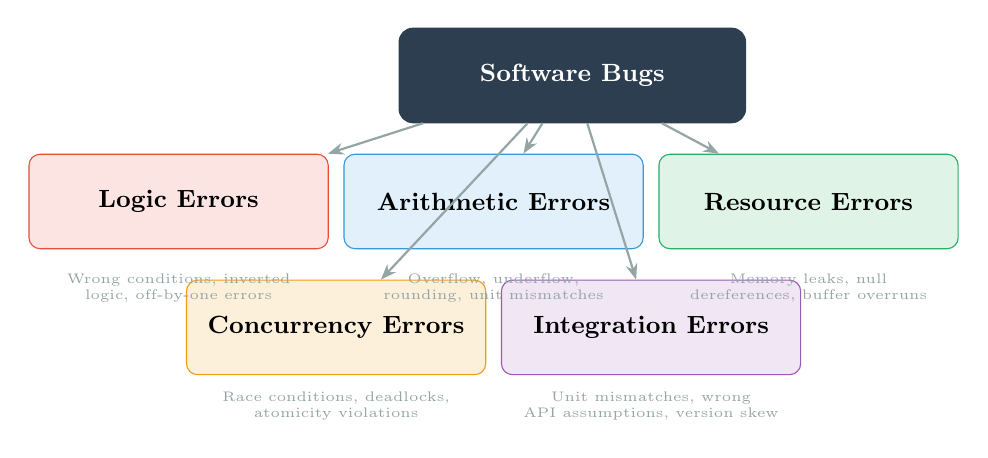
\begin{tikzpicture}[
    root/.style={rectangle, rounded corners=5pt, draw=csprimary, fill=csprimary,
                 minimum width=44mm, minimum height=12mm, align=center,
                 font=\small\bfseries\color{white}},
    cat/.style={rectangle, rounded corners=4pt, draw=#1, fill=#1!15,
                minimum width=38mm, minimum height=12mm, align=center,
                font=\small\bfseries},
    arrow/.style={-{Stealth[length=2mm]}, thick, color=codegray}
]
\node[root] (bugs) at (5,4) {Software Bugs};

\node[cat=cssecondary]  (logic)   at (0,2.4)    {Logic Errors};
\node[cat=cstertiary]   (arith)   at (4,2.4)    {Arithmetic Errors};
\node[cat=csaccent]     (resource) at (8,2.4)   {Resource Errors};
\node[cat=cswarm]       (concur)  at (2,0.8)    {Concurrency Errors};
\node[cat=codepurple]   (integr)  at (6,0.8)    {Integration Errors};

\draw[arrow] (bugs) -- (logic);
\draw[arrow] (bugs) -- (arith);
\draw[arrow] (bugs) -- (resource);
\draw[arrow] (bugs) -- (concur);
\draw[arrow] (bugs) -- (integr);

\node[font=\tiny, color=codegray, align=center, text width=36mm] at (0,1.3)
    {Wrong conditions, inverted\\logic, off-by-one errors};
\node[font=\tiny, color=codegray, align=center, text width=36mm] at (4,1.3)
    {Overflow, underflow,\\rounding, unit mismatches};
\node[font=\tiny, color=codegray, align=center, text width=36mm] at (8,1.3)
    {Memory leaks, null\\dereferences, buffer overruns};
\node[font=\tiny, color=codegray, align=center, text width=36mm] at (2,-0.2)
    {Race conditions, deadlocks,\\atomicity violations};
\node[font=\tiny, color=codegray, align=center, text width=36mm] at (6,-0.2)
    {Unit mismatches, wrong\\API assumptions, version skew};
\end{tikzpicture}
\end{center}

Each category has its own character---and its own testing challenges. Logic errors can often be found by carefully testing the boundary cases of conditions. Arithmetic errors require attention to data types and ranges. Concurrency errors may appear only under specific timing conditions and can be nearly impossible to reproduce reliably.

%---------- FAMOUS BUGS ----------%
\section{A History of Famous Bugs}

The history of software bugs is also a history of the consequences of getting things wrong---from mildly annoying to catastrophic.

\begin{historybox}[Mariner 1: The Missing Hyphen (1962)]
NASA's Mariner 1 was designed to be the first spacecraft to fly past Venus. Shortly after launch in July 1962, the rocket began veering off course. The range safety officer destroyed the vehicle 293 seconds into flight at a cost of approximately \$80 million (over \$700 million in today's dollars).

The cause: a transcription error when converting a handwritten formula to computer code. A single overbar symbol (indicating a smoothed average) was omitted from the FORTRAN guidance program. Without it, the software used raw velocity data instead of filtered data, causing it to overcorrect for normal fluctuations.

Author Arthur C.\ Clarke called it ``the most expensive hyphen in history.'' It is a canonical example of how a tiny, invisible error in code can have enormous real-world consequences.
\end{historybox}

\begin{historybox}[Therac-25: When Bugs Kill (1985--1987)]
The Therac-25 was a radiation therapy machine used to treat cancer. Between 1985 and 1987, it delivered massive radiation overdoses to at least six patients. Three died. The others suffered severe radiation burns.

The cause was a \keyterm{race condition}---a class of concurrency bug in which the result of a computation depends on the precise timing of events. The Therac-25's control software had been adapted from an earlier model that had hardware safety interlocks. When those interlocks were removed to reduce cost, the software's timing-dependent safety checks were exposed. A trained operator who typed quickly could enter a sequence of commands that, by a matter of milliseconds, bypassed the safety checks and activated the high-power beam without the beam-shaping hardware in place.

The Therac-25 case is studied in every software engineering ethics course because it illustrates that software bugs are not merely technical problems---they have human consequences, and the engineers and institutions responsible for safety-critical software bear genuine moral responsibility.
\end{historybox}

\begin{historybox}[Ariane 5: The Overflow Disaster (1996)]
The European Space Agency's Ariane 5 rocket exploded 37 seconds after launch in June 1996, destroying four satellites worth approximately \$370 million.

The cause: an \keyterm{integer overflow}. A 64-bit floating-point value representing the rocket's horizontal velocity was converted to a 16-bit integer. The value was too large to fit---it exceeded the maximum a 16-bit integer can hold---and caused a hardware exception. The backup navigation computer, running identical software, failed in the same way. The primary flight computer, receiving garbage data, shut itself down. The rocket, receiving no guidance, self-destructed.

The irony: the overflowing variable tracked horizontal velocity during a ground alignment phase. On Ariane 5, this value was always large because the rocket launched from a different location than Ariane 4. The code had been reused from Ariane 4 without analyzing whether its assumptions still held. Reusing code without understanding its assumptions is a recurring theme in software disasters.
\end{historybox}

\begin{historybox}[The Mars Climate Orbiter: Units Matter (1999)]
The Mars Climate Orbiter was a \$327 million NASA spacecraft designed to study the Martian climate. On September 23, 1999, it fired its engine to enter Mars orbit. The trajectory was slightly wrong, and the spacecraft either burned up in the atmosphere or skipped off it into space.

The cause: one engineering team was transmitting thruster force data in pound-force seconds; the receiving software expected newton-seconds. The two units differ by a factor of 4.45. Over the nine-month journey, the small error accumulated until the trajectory was fatally off.

This is not a programming bug in the narrow sense---the individual programs worked correctly. It is an \textit{interface} bug: a mismatch in assumptions between components, undocumented and unchecked. Integration bugs of this type are among the hardest to catch because each component, tested in isolation, behaves correctly.
\end{historybox}

\begin{historybox}[Knight Capital: 45 Minutes and \$440 Million (2012)]
Knight Capital Group was one of the largest US equity market makers. On August 1, 2012, a technician deployed new trading software to seven of eight production servers but forgot the eighth. The forgotten server was running old code that included a dormant feature called ``Power Peg'' that had been deactivated years earlier but never removed from the codebase.

When the market opened, Knight's system began executing thousands of unintended trades per second. The dormant code on the eighth server was activated by new message types and began buying high and selling low---the worst possible trading strategy---at machine speed. In 45 minutes, Knight lost \$440 million. The company never recovered and was acquired months later.

The deployment failure was caused by a manual process with no automated verification that all servers had received identical code. A single absent checkbox in a release script ended a firm.
\end{historybox}

\begin{historybox}[Boeing 737 MAX: Software and the Cost of Secrecy (2018--2019)]
The Boeing 737 MAX was designed with larger engines mounted further forward than previous 737 models, which altered the aircraft's handling characteristics. To avoid expensive pilot retraining, Boeing developed the \textbf{MCAS} (Maneuvering Characteristics Augmentation System): software that automatically pushed the nose down if sensors detected a high angle of attack.

MCAS read from a single angle-of-attack sensor. If that sensor failed or gave erroneous readings, MCAS would push the nose down regardless of the pilot's inputs---and the published pilot training materials did not mention MCAS existed. On Lion Air flight 610 (October 2018) and Ethiopian Airlines flight 302 (March 2019), faulty sensor data triggered MCAS. Pilots unfamiliar with a system they didn't know existed could not stop it. 346 people died.

The technical failure was real: MCAS lacked sensor redundancy and failed-safe behavior. But the deeper failure was institutional: regulatory certification shortcuts, economic pressure, and the decision to conceal the system's existence from pilots who might otherwise have refused to fly without additional training.
\end{historybox}

%---------- POPPER AND DIJKSTRA ----------%
\section{The Philosophy of Testing: Popper and Dijkstra}

\subsection{Karl Popper and Falsificationism}

In the 1930s, philosopher Karl Popper tackled a fundamental question: what separates science from non-science? His answer was \keyterm{falsifiability}: a claim is scientific if and only if it is possible to specify an observation that would prove it \textit{wrong}.

This might seem backwards. Shouldn't science be about proving things \textit{right}? Popper's insight was that no number of confirming observations can \textit{prove} a universal claim. You can observe a million white swans and conclude ``all swans are white''---but one black swan refutes the claim forever. Confirmation accumulates; a single falsification destroys.

\begin{quotebox}[Karl Popper --- \textit{The Logic of Scientific Discovery} (1934)]
``It must be possible for an empirical scientific system to be refuted by experience\ldots\ I shall not require of a scientific system that it shall be capable of being singled out, once and for all, in a positive sense; but I shall require that its logical form shall be such that it can be singled out, in a negative sense: it must be possible for an empirical scientific system to be refuted by experience.''
\end{quotebox}

The asymmetry is fundamental: \textit{confirmation is weak; falsification is strong.} A thousand passing tests suggest (but do not prove) correctness. One failing test proves a bug beyond doubt.

\subsection{Dijkstra's Corollary}

Edsger W.\ Dijkstra, one of the towering figures of computer science, applied this insight directly to software testing in 1969:

\begin{quotebox}[Edsger W.\ Dijkstra --- ``Notes on Structured Programming'' (1969)]
``Program testing can be used to show the presence of bugs, but never to show their absence!''
\end{quotebox}

The exclamation mark is his. Dijkstra was not being dramatic---he was stating a logical consequence of the structure of software. A program with even modest complexity can be executed in a combinatorially enormous number of ways. A function that takes a 32-bit integer as input has over four billion possible inputs. Testing them all is generally impossible. No finite test suite can cover all possible executions of a non-trivial program.

\begin{center}
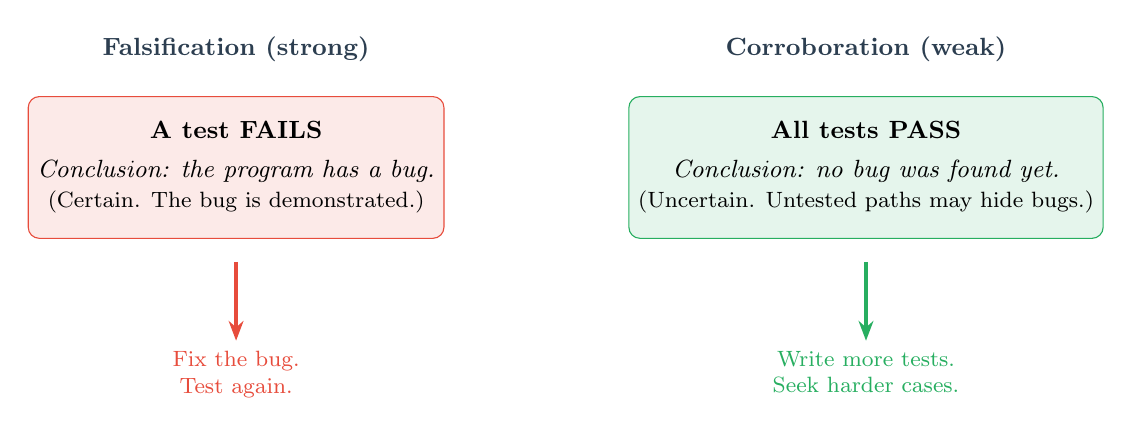
\begin{tikzpicture}[
    box/.style={rectangle, rounded corners=4pt, draw=#1, fill=#1!12,
                minimum width=52mm, minimum height=18mm, align=center, font=\small},
    arrow/.style={-{Stealth[length=2.5mm]}, very thick}
]
\node[box=cssecondary] (fail) at (0,0)
    {\textbf{A test FAILS}\\[3pt]
     \textit{Conclusion: the program has a bug.}\\
     \footnotesize (Certain. The bug is demonstrated.)};

\node[box=csaccent] (pass) at (8,0)
    {\textbf{All tests PASS}\\[3pt]
     \textit{Conclusion: no bug was found yet.}\\
     \footnotesize (Uncertain. Untested paths may hide bugs.)};

\node[font=\small\bfseries, color=csprimary] at (0, 1.5) {Falsification (strong)};
\node[font=\small\bfseries, color=csprimary] at (8, 1.5) {Corroboration (weak)};

\draw[arrow, color=cssecondary] (0, -1.2) -- (0, -2.2)
    node[below, font=\footnotesize, color=cssecondary, align=center]
    {Fix the bug.\\Test again.};

\draw[arrow, color=csaccent] (8, -1.2) -- (8, -2.2)
    node[below, font=\footnotesize, color=csaccent, align=center]
    {Write more tests.\\Seek harder cases.};
\end{tikzpicture}
\end{center}

\subsection{What This Means in Practice}

The Popper--Dijkstra insight reshapes how a thoughtful programmer approaches testing:

\begin{itemize}[itemsep=4pt]
    \item \textbf{Tests can never be ``done.''} Passing a test suite means you haven't found a bug in the tested paths---not that no bugs exist in untested paths. Seeking harder, more adversarial test cases is always worthwhile.

    \item \textbf{Each failing test is a gift.} A failing test reveals a real bug. The discomfort of a red test result is the system working as intended.

    \item \textbf{Test the boundaries.} Most bugs lurk at the edges---the off-by-one error, the empty list, the negative number, the maximum value, the null input. Testing typical inputs tells you the program works in typical cases; testing boundary inputs tells you it handles the exceptional cases that are most likely to hide bugs.

    \item \textbf{Tests as specifications.} A test suite doubles as an executable specification of what a program is supposed to do. A test that says \texttt{assertEquals(4, add(2, 2))} is both a check and a statement of intent.
\end{itemize}

\begin{debatebox}[Can We Ever Prove Correctness?]
Dijkstra himself believed the answer was yes---but not through testing. He championed \textbf{formal verification}: using mathematical proof to establish that a program meets its specification for \textit{all} possible inputs.

Formal methods are used in safety-critical domains: the Paris M\'{e}tro Line 14 (driverless), aircraft autopilot systems, cryptographic protocols, and microprocessor designs. The \textbf{seL4 microkernel}---used in aerospace and defense systems---is formally verified: every line of code has been mathematically proven correct.

But formal verification is expensive and technically demanding. It requires specifying precisely what ``correct'' means, which is harder than it sounds. And a proof is only as good as the specification---if the specification itself is wrong, the proof is useless.

For most software, formal verification is impractical. For software where bugs can kill people, it may be the only responsible choice.
\end{debatebox}

%---------- UNIT TESTING IN JAVA ----------%
\section{Unit Testing in Java with JUnit}

\subsection{What is a Unit Test?}

A \keyterm{unit test} is a piece of code that tests one small, specific piece of behavior (a ``unit''---typically one method) in isolation from the rest of the program. Unit tests are:

\begin{itemize}[itemsep=3pt]
    \item \textbf{Automated:} They run without human intervention and report pass or fail.
    \item \textbf{Fast:} Hundreds of unit tests should run in seconds.
    \item \textbf{Isolated:} Each test checks one thing; failures are easy to localize.
    \item \textbf{Repeatable:} Running them again always gives the same result.
\end{itemize}

\textbf{JUnit} is the standard unit testing framework for Java. It is included in most Java IDEs and build tools. A JUnit test is a regular Java class with methods marked with the \texttt{@Test} annotation.

\subsection{A First Example: Testing a Buggy Method}

Let's start with a deliberately flawed method---a function to compute the average of an array of integers---and see how tests reveal the bugs.

\begin{bugcode}[A Buggy average() Method --- Can You Spot the Bugs?]
public class Statistics {

    // Returns the average of the values in the array.
    public static double average(int[] values) {
        int sum = 0;
        for (int i = 0; i <= values.length; i++) {   // BUG 1
            sum += values[i];
        }
        return sum / values.length;                  // BUG 2
    }
}
\end{bugcode}

There are two bugs here. Can you find them before reading on?

\begin{itemize}[itemsep=3pt]
    \item \textbf{Bug 1:} The loop condition is \texttt{i <= values.length} instead of \texttt{i < values.length}. This is an \textit{off-by-one error}: on the last iteration, \texttt{values[values.length]} is accessed, which is beyond the end of the array. Java throws an \texttt{ArrayIndexOutOfBoundsException}.
    \item \textbf{Bug 2:} \texttt{sum / values.length} is \textit{integer division} when both operands are \texttt{int}. The average of \{1, 2\} would compute as \texttt{3 / 2 = 1}, not \texttt{1.5}.
\end{itemize}

Now let's write JUnit tests that expose both bugs:

\begin{javacode}[JUnit Tests That Reveal the Bugs]
import org.junit.jupiter.api.Test;
import static org.junit.jupiter.api.Assertions.*;

public class StatisticsTest {

    // A normal case: should work for typical input
    @Test
    void averageOfThreeValues() {
        double result = Statistics.average(new int[]{2, 4, 6});
        assertEquals(4.0, result, 1e-9);
    }

    // Tests fractional result --- exposes Bug 2 (integer division)
    @Test
    void averageProducesFractionalResult() {
        double result = Statistics.average(new int[]{1, 2});
        assertEquals(1.5, result, 1e-9);  // FAILS: returns 1.0
    }

    // Single element --- also exposes Bug 1 via crash
    @Test
    void averageOfOneValue() {
        double result = Statistics.average(new int[]{42});
        assertEquals(42.0, result, 1e-9); // FAILS: ArrayIndexOutOfBoundsException
    }

    // Edge case: all the same value
    @Test
    void averageOfIdenticalValues() {
        double result = Statistics.average(new int[]{7, 7, 7, 7});
        assertEquals(7.0, result, 1e-9);
    }

    // Edge case: negative numbers
    @Test
    void averageWithNegatives() {
        double result = Statistics.average(new int[]{-3, -1, 1, 3});
        assertEquals(0.0, result, 1e-9);
    }

    // Edge case: what should happen with an empty array?
    @Test
    void averageOfEmptyArrayThrowsException() {
        assertThrows(IllegalArgumentException.class,
                     () -> Statistics.average(new int[]{}));
    }
}
\end{javacode}

\begin{tipbox}[Reading the assertEquals arguments]
\texttt{assertEquals(expected, actual, delta)} takes three arguments:
\begin{enumerate}[itemsep=1pt]
    \item \textbf{expected} --- what you calculated the correct answer should be
    \item \textbf{actual} --- what the method actually returned
    \item \textbf{delta} --- tolerance for floating-point comparison (\texttt{1e-9} means they must agree to 9 decimal places)
\end{enumerate}
Always put expected first and actual second. When a test fails, JUnit prints ``expected $\langle$X$\rangle$ but was $\langle$Y$\rangle$''---this only makes sense if you follow the convention.
\end{tipbox}

Now let's write the corrected method, informed by the failing tests:

\begin{javacode}[The Corrected average() Method]
public class Statistics {

    public static double average(int[] values) {
        if (values == null || values.length == 0) {
            throw new IllegalArgumentException(
                "Cannot compute average of empty array");
        }

        long sum = 0;                               // long avoids overflow
        for (int i = 0; i < values.length; i++) {  // < not <=
            sum += values[i];
        }
        return (double) sum / values.length;        // cast forces double division
    }
}
\end{javacode}

Running the same test suite against the fixed method: all six tests pass. Notice that the test for the empty array (which previously would have caused a \texttt{/ by zero} error) now passes because we explicitly handle that case.

\subsection{The Ariane 5 Bug in Java}

Let's recreate the integer overflow that destroyed the Ariane 5 rocket, this time in Java:

\begin{bugcode}[Recreating the Ariane 5 Overflow in Java]
public class NavigationSystem {

    // Converts a velocity (as a double) to a 16-bit short for the legacy
    // navigation computer. DANGER: no range checking!
    public static short velocityToShort(double velocity) {
        return (short) velocity;  // Silent data corruption if out of range!
    }

    public static void main(String[] args) {
        // Ariane 4 scenario: horizontal velocity stays small
        double ariane4Velocity = 15000.0;
        System.out.println("Ariane 4 velocity: " + velocityToShort(ariane4Velocity));
        // Prints: 15000  (correct)

        // Ariane 5 scenario: much higher horizontal velocity due to launch site
        double ariane5Velocity = 37000.0;
        System.out.println("Ariane 5 velocity: " + velocityToShort(ariane5Velocity));
        // Prints: 1464  (WRONG! Short.MAX_VALUE is 32767; 37000 overflows silently)
    }
}
\end{bugcode}

\begin{javacode}[Tests That Would Have Caught the Overflow]
@Test
void velocityConversionInRange() {
    assertEquals((short)15000, NavigationSystem.velocityToShort(15000.0));
}

@Test
void velocityConversionThrowsOnOverflow() {
    // This test fails against the original code ---
    // it just silently returns a wrong value.
    // The fix requires adding a range check.
    assertThrows(ArithmeticException.class,
                 () -> NavigationSystem.velocityToShort(37000.0));
}
\end{javacode}

The second test reveals the gap: without the \texttt{assertThrows}, a test of \texttt{velocityToShort(37000.0)} would \textit{pass} (it returns \texttt{1464} without complaint), giving false confidence.

\begin{tipbox}[Testing for Failure Is as Important as Testing for Success]
Many beginning programmers write tests only for the ``happy path''---the expected, normal inputs. But bugs most often hide in:
\begin{itemize}[itemsep=2pt]
    \item \textbf{Boundary values:} the minimum and maximum legal inputs
    \item \textbf{Just outside boundaries:} one less than minimum; one more than maximum
    \item \textbf{Special values:} zero, negative numbers, \texttt{null}, empty strings or arrays
    \item \textbf{Error cases:} inputs that should cause an exception
\end{itemize}
A test that checks \texttt{divide(10, 2) == 5} is useful. A test that checks \texttt{divide(10, 0)} throws an exception is \textit{more} useful---because division by zero is exactly the case that production code is likely to receive and that a programmer might forget to handle.
\end{tipbox}

%---------- TDD ----------%
\section{Test-Driven Development}

\subsection{Reversing the Order}

The natural impulse is to write code first and tests afterward. \keyterm{Test-driven development} (TDD) reverses this: you write the test \textit{before} you write the code it tests.

The TDD workflow follows a simple three-phase cycle:

\begin{center}
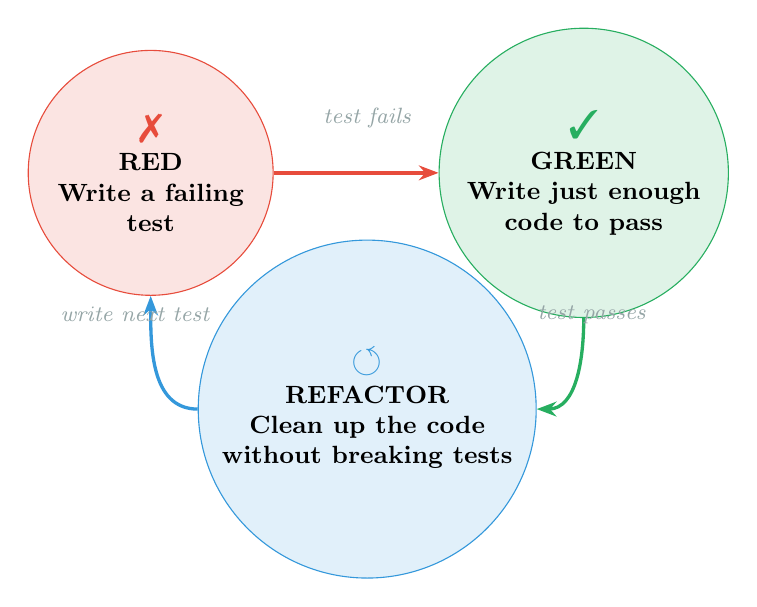
\begin{tikzpicture}[
    phase/.style={circle, draw=#1, fill=#1!15, minimum size=28mm, align=center, font=\small\bfseries},
    arrow/.style={-{Stealth[length=2.5mm]}, very thick}
]
\node[phase=cssecondary] (red)    at (0,0)    {\textcolor{cssecondary}{\Large\ding{55}}\\RED\\Write a failing\\test};
\node[phase=csaccent]    (green)  at (5.5,0)  {\textcolor{csaccent}{\Large\ding{51}}\\GREEN\\Write just enough\\code to pass};
\node[phase=cstertiary]  (refact) at (2.75,-3){\textcolor{cstertiary}{\Large$\circlearrowleft$}\\REFACTOR\\Clean up the code\\without breaking tests};

\draw[arrow, color=cssecondary] (red.east)   -- (green.west);
\draw[arrow, color=csaccent]    (green.south) to[out=-90, in=0] (refact.east);
\draw[arrow, color=cstertiary]  (refact.west) to[out=180, in=-90] (red.south);

\node[font=\footnotesize\itshape, color=codegray] at (2.75, 0.7) {test fails};
\node[font=\footnotesize\itshape, color=codegray] at (5.6,-1.8) {test passes};
\node[font=\footnotesize\itshape, color=codegray] at (-0.2,-1.8) {write next test};
\end{tikzpicture}
\end{center}

\subsection{TDD in Practice: Building a GradeBook}

Let's build a simple \texttt{GradeBook} class using TDD. We start with no implementation---just tests that describe the behavior we want.

\begin{javacode}[Step 1: Write Failing Tests First]
import org.junit.jupiter.api.BeforeEach;
import org.junit.jupiter.api.Test;
import static org.junit.jupiter.api.Assertions.*;

public class GradeBookTest {
    private GradeBook book;

    @BeforeEach
    void setUp() {
        book = new GradeBook();  // Does not exist yet -- won't compile!
    }

    @Test
    void newGradeBookIsEmpty() {
        assertEquals(0, book.getCount());
    }

    @Test
    void addingGradeIncreasesCount() {
        book.addGrade(85.0);
        assertEquals(1, book.getCount());
    }

    @Test
    void averageOfOneGrade() {
        book.addGrade(90.0);
        assertEquals(90.0, book.getAverage(), 1e-9);
    }

    @Test
    void averageOfMultipleGrades() {
        book.addGrade(70.0);
        book.addGrade(80.0);
        book.addGrade(90.0);
        assertEquals(80.0, book.getAverage(), 1e-9);
    }

    @Test
    void highestGrade() {
        book.addGrade(72.0);
        book.addGrade(95.0);
        book.addGrade(88.0);
        assertEquals(95.0, book.getHighest(), 1e-9);
    }

    @Test
    void averageOfEmptyBookThrowsException() {
        assertThrows(IllegalStateException.class, () -> book.getAverage());
    }
}
\end{javacode}

\begin{javacode}[Step 2: Write the Minimum Code to Make Tests Pass]
import java.util.ArrayList;
import java.util.List;

public class GradeBook {
    private List<Double> grades = new ArrayList<>();

    public void addGrade(double grade) {
        grades.add(grade);
    }

    public int getCount() {
        return grades.size();
    }

    public double getAverage() {
        if (grades.isEmpty()) {
            throw new IllegalStateException("No grades recorded");
        }
        double sum = 0;
        for (double g : grades) sum += g;
        return sum / grades.size();
    }

    public double getHighest() {
        if (grades.isEmpty()) {
            throw new IllegalStateException("No grades recorded");
        }
        double max = grades.get(0);
        for (double g : grades) {
            if (g > max) max = g;
        }
        return max;
    }
}
\end{javacode}

All six tests now pass. The tests specified the behavior; the implementation fulfilled it.

\begin{tipbox}[Why TDD Produces Better Code]
TDD has practical benefits beyond correctness:

\textbf{Forces you to think before you code.} Writing a test requires knowing what the method \textit{should} do---the input, the expected output, and the edge cases. This thinking often reveals ambiguities or design problems before any code is written.

\textbf{Produces naturally testable code.} Code written test-first tends to have small methods with clear inputs and outputs---because that's what's easy to test. Code written implementation-first often has tangled dependencies that are difficult to test afterward.

\textbf{Provides a safety net for changes.} When you later modify the \texttt{GradeBook}---adding letter grades, weighting categories---the existing tests immediately tell you if you've broken existing behavior. This is called \keyterm{regression testing}.

\textbf{Documents intent.} The test suite documents what the code is \textit{supposed} to do, in executable form. New team members can read the tests to understand the expected behavior.
\end{tipbox}

%---------- BEYOND UNIT TESTS ----------%
\section{Beyond Unit Tests: A Testing Vocabulary}

Unit tests are essential but not sufficient. A complete testing strategy layers several complementary approaches:

\begin{center}
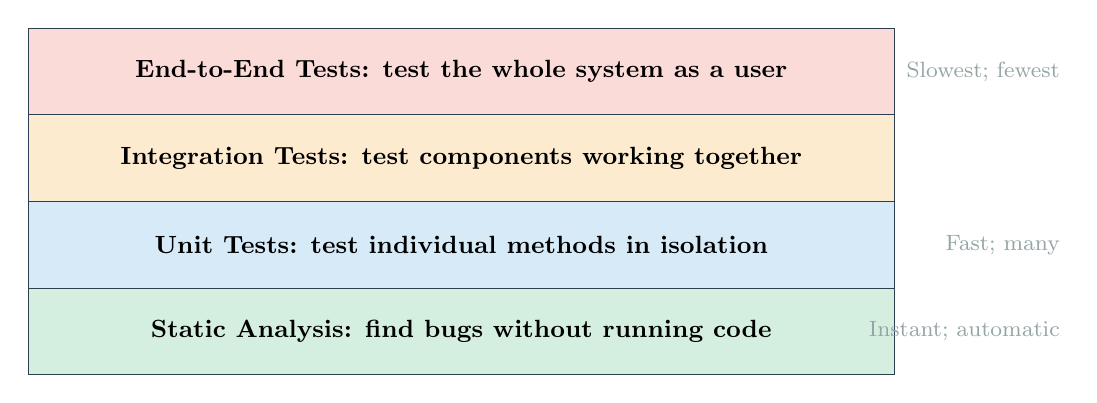
\begin{tikzpicture}[
    layer/.style={rectangle, draw=csprimary, fill=#1,
                  minimum width=110mm, minimum height=11mm,
                  align=center, font=\small\bfseries},
    lbl/.style={font=\footnotesize, color=codegray, align=right, text width=28mm}
]
\node[layer=cssecondary!20]  (e2e)    at (0, 3.3) {End-to-End Tests: test the whole system as a user};
\node[layer=cswarm!20]       (integ)  at (0, 2.2) {Integration Tests: test components working together};
\node[layer=cstertiary!20]   (unit)   at (0, 1.1) {Unit Tests: test individual methods in isolation};
\node[layer=csaccent!20]     (static) at (0, 0.0) {Static Analysis: find bugs without running code};

\node[lbl] at (6.2, 3.3) {Slowest; fewest};
\node[lbl] at (6.2, 2.2) {};
\node[lbl] at (6.2, 1.1) {Fast; many};
\node[lbl] at (6.2, 0.0) {Instant; automatic};
\end{tikzpicture}
\end{center}

\textbf{Integration tests} verify that separately correct components work correctly \textit{together}. The Mars Climate Orbiter failure was an integration bug: each team's software was correct in isolation. Integration tests would have verified that the units produced by one team were interpretable by the other.

\textbf{End-to-end tests} simulate real user scenarios through the complete system. They catch bugs that only emerge when all the pieces interact, but they are slower and more fragile than unit tests.

\textbf{Static analysis} tools examine source code without running it, looking for common bug patterns: unused variables, unreachable code, potential null dereferences, and type mismatches. Java's compiler itself performs basic static analysis. Tools like \textbf{SpotBugs} and \textbf{PMD} go further. Some languages (notably Rust) have static analysis so thorough that entire categories of bugs---null pointer errors, data races---are ruled out at compile time.

\textbf{Property-based testing} generates \textit{random} inputs and tests that high-level properties hold for all of them---a powerful extension of the Popperian approach. Instead of writing specific test cases, you specify invariants: ``the average should always be between the minimum and maximum,'' ``sorting should never change the list's size.'' The framework then tries thousands of random inputs trying to find a counterexample.

%---------- THE HUMAN SIDE ----------%
\section{The Human Side of Bugs}

\subsection{Blameless Postmortems}

When a significant bug reaches production and causes harm, the instinctive response is to find the person who made the mistake and hold them accountable. This instinct is understandable but counterproductive.

Modern software engineering culture has increasingly adopted the \keyterm{blameless postmortem}: a structured analysis of what went wrong that focuses on \textit{systemic} causes rather than individual culpability. The reasoning is straightforward:

\begin{itemize}[itemsep=3pt]
    \item Software is too complex for any individual to understand completely. Bugs are almost always the result of multiple contributing factors.
    \item Engineers who fear punishment for mistakes hide them or avoid taking on risky work. A culture of psychological safety produces better outcomes.
    \item Fixing the \textit{system} that allowed the bug to exist prevents similar bugs in the future. Blaming an individual does nothing to fix the system.
\end{itemize}

\begin{debatebox}[Individual Responsibility vs.\ System Failure]
The blameless postmortem approach has limits. Engineers on the Therac-25 ignored user reports of problems, dismissed error messages as display glitches, and deployed software they had not adequately tested for safety-critical use. The Boeing 737 MAX failures involved corporate decisions to conceal the MCAS system from pilots. In cases where individuals or organizations were reckless or dishonest, systemic framing can become a shield against deserved accountability.

A thoughtful position: most bugs emerge from systems, not malice or unique incompetence. But when individuals choose to cut corners, suppress safety concerns, or make decisions they know to be dangerous for financial gain, individual accountability is appropriate alongside systemic analysis. The question is not ``blame or no blame'' but ``what causal story most accurately describes what happened, and what response would best prevent recurrence?''
\end{debatebox}

\subsection{Bug Reporting and Reproduction}

A bug that cannot be reproduced cannot be fixed. When reporting a bug---to a colleague, to an open-source project, or in your own notes---the essential ingredients are:

\begin{enumerate}[itemsep=3pt]
    \item \textbf{Steps to reproduce:} Precisely what actions or inputs trigger the bug.
    \item \textbf{Expected behavior:} What the program \textit{should} have done.
    \item \textbf{Actual behavior:} What the program \textit{did} instead, including any error messages.
    \item \textbf{Environment:} Language version, operating system, relevant configuration.
\end{enumerate}

A test that reliably reproduces the bug is the gold standard of a bug report. Before filing a bug report, write a unit test that fails because of the bug. When the bug is fixed, the test passes---and stays in the test suite to prevent regression.

%---------- DISCUSSION QUESTIONS ----------%
\section*{Discussion Questions}

\begin{questionbox}
\begin{enumerate}[leftmargin=*, label=\textcolor{cswarm}{\textbf{\arabic*.}}]
    \item \textbf{Popper and Testing:} Popper argued that no number of confirming observations proves a theory; one counterexample refutes it. How does this apply to software testing? If you run 10{,}000 tests and all pass, what have you learned? What haven't you learned? Does this make testing feel less valuable to you---or more?

    \item \textbf{The Ariane 5 Lesson:} The Ariane 5 failure was caused by reusing code from Ariane 4 without analyzing whether its assumptions still held. Can you think of other contexts---outside of rocketry---where reusing something without checking its assumptions could cause serious problems?

    \item \textbf{Therac-25 and Moral Responsibility:} The Therac-25 killed people because of a software bug. Who bears moral responsibility: the individual programmers who wrote the faulty code? The managers who removed hardware interlocks to reduce cost? The hospital administrators who purchased and deployed the machine? The regulators who approved it? How should responsibility be distributed in complex sociotechnical systems?

    \item \textbf{TDD Trade-offs:} Test-driven development requires writing tests before writing implementation code. What would be the advantages of this approach in a student project? What would be the disadvantages? Under what circumstances might TDD be impractical?

    \item \textbf{The Limits of Testing:} Dijkstra said testing can show the presence of bugs but never their absence. Does this mean we should pursue formal verification for all software? What would be the costs and benefits of requiring mathematically verified software for any system where lives are at stake?
\end{enumerate}
\end{questionbox}

%---------- GLOSSARY ----------%
\section*{Key Terms}

\begin{glossarybox}
\begin{description}[leftmargin=!, labelwidth=3.8cm, font=\bfseries\color{cssecondary}]
    \item[Blameless Postmortem] A structured analysis of a failure that focuses on systemic and process causes rather than individual blame, to enable learning and prevent recurrence.

    \item[Boundary Value] An input at the edge of a valid range (the minimum, the maximum, or just beyond either); bugs disproportionately hide at boundaries.

    \item[Edge Case] An input or condition at an extreme or unusual corner of a function's domain; often the last cases tested and the first to harbor bugs.

    \item[Falsifiability] Karl Popper's criterion for scientific claims: a claim is scientific only if it can in principle be refuted by observation; the asymmetry between confirmation and falsification.

    \item[Formal Verification] Mathematically proving that a program satisfies its specification for all possible inputs, as opposed to testing a finite sample of inputs.

    \item[Integer Overflow] A bug where an arithmetic result exceeds the maximum value that can be stored in the chosen integer type, producing a silently incorrect result.

    \item[JUnit] The standard Java unit testing framework; provides annotations (\texttt{@Test}) and assertion methods (\texttt{assertEquals}) for writing automated tests.

    \item[Off-by-One Error] A logic error where a loop or index is one position too far or too short; among the most common bugs in all of programming.

    \item[Race Condition] A concurrency bug where the outcome depends on the relative timing of events in different execution threads; can produce different results on different runs.

    \item[Regression Testing] Running an existing test suite after making changes to a program, to verify that previously working behavior has not been broken.

    \item[Software Bug] Any flaw in a program that causes it to produce incorrect behavior, crash, or otherwise deviate from its specification.

    \item[Static Analysis] Examining source code without running it to find potential bugs, style violations, or security vulnerabilities.

    \item[Test-Driven Development] A development practice in which tests are written before the implementation code they test, following a Red--Green--Refactor cycle.

    \item[Unit Test] An automated test that checks one small unit of behavior (typically one method) in isolation from the rest of the system.
\end{description}
\end{glossarybox}

\vspace{5mm}

%---------- FOOTER ----------%
\begin{center}
\textcolor{csprimary}{\rule{0.6\textwidth}{0.5pt}}\\[3mm]
{\small\textcolor{gray}{This case study is part of the Open Educational Resources for \cscourse.\\
Licensed under Creative Commons Attribution 4.0 (CC BY 4.0).}}
\end{center}

\end{document}
